\section{服务生态系统与面向服务的计算}

\subsection{服务生态系统}

面向服务的应用逻辑,遵循面向服务的设计原则,采用服务和服务组合加以实现。

\begin{figure}[H]
    \vspace{-0.5em}
	\centering
	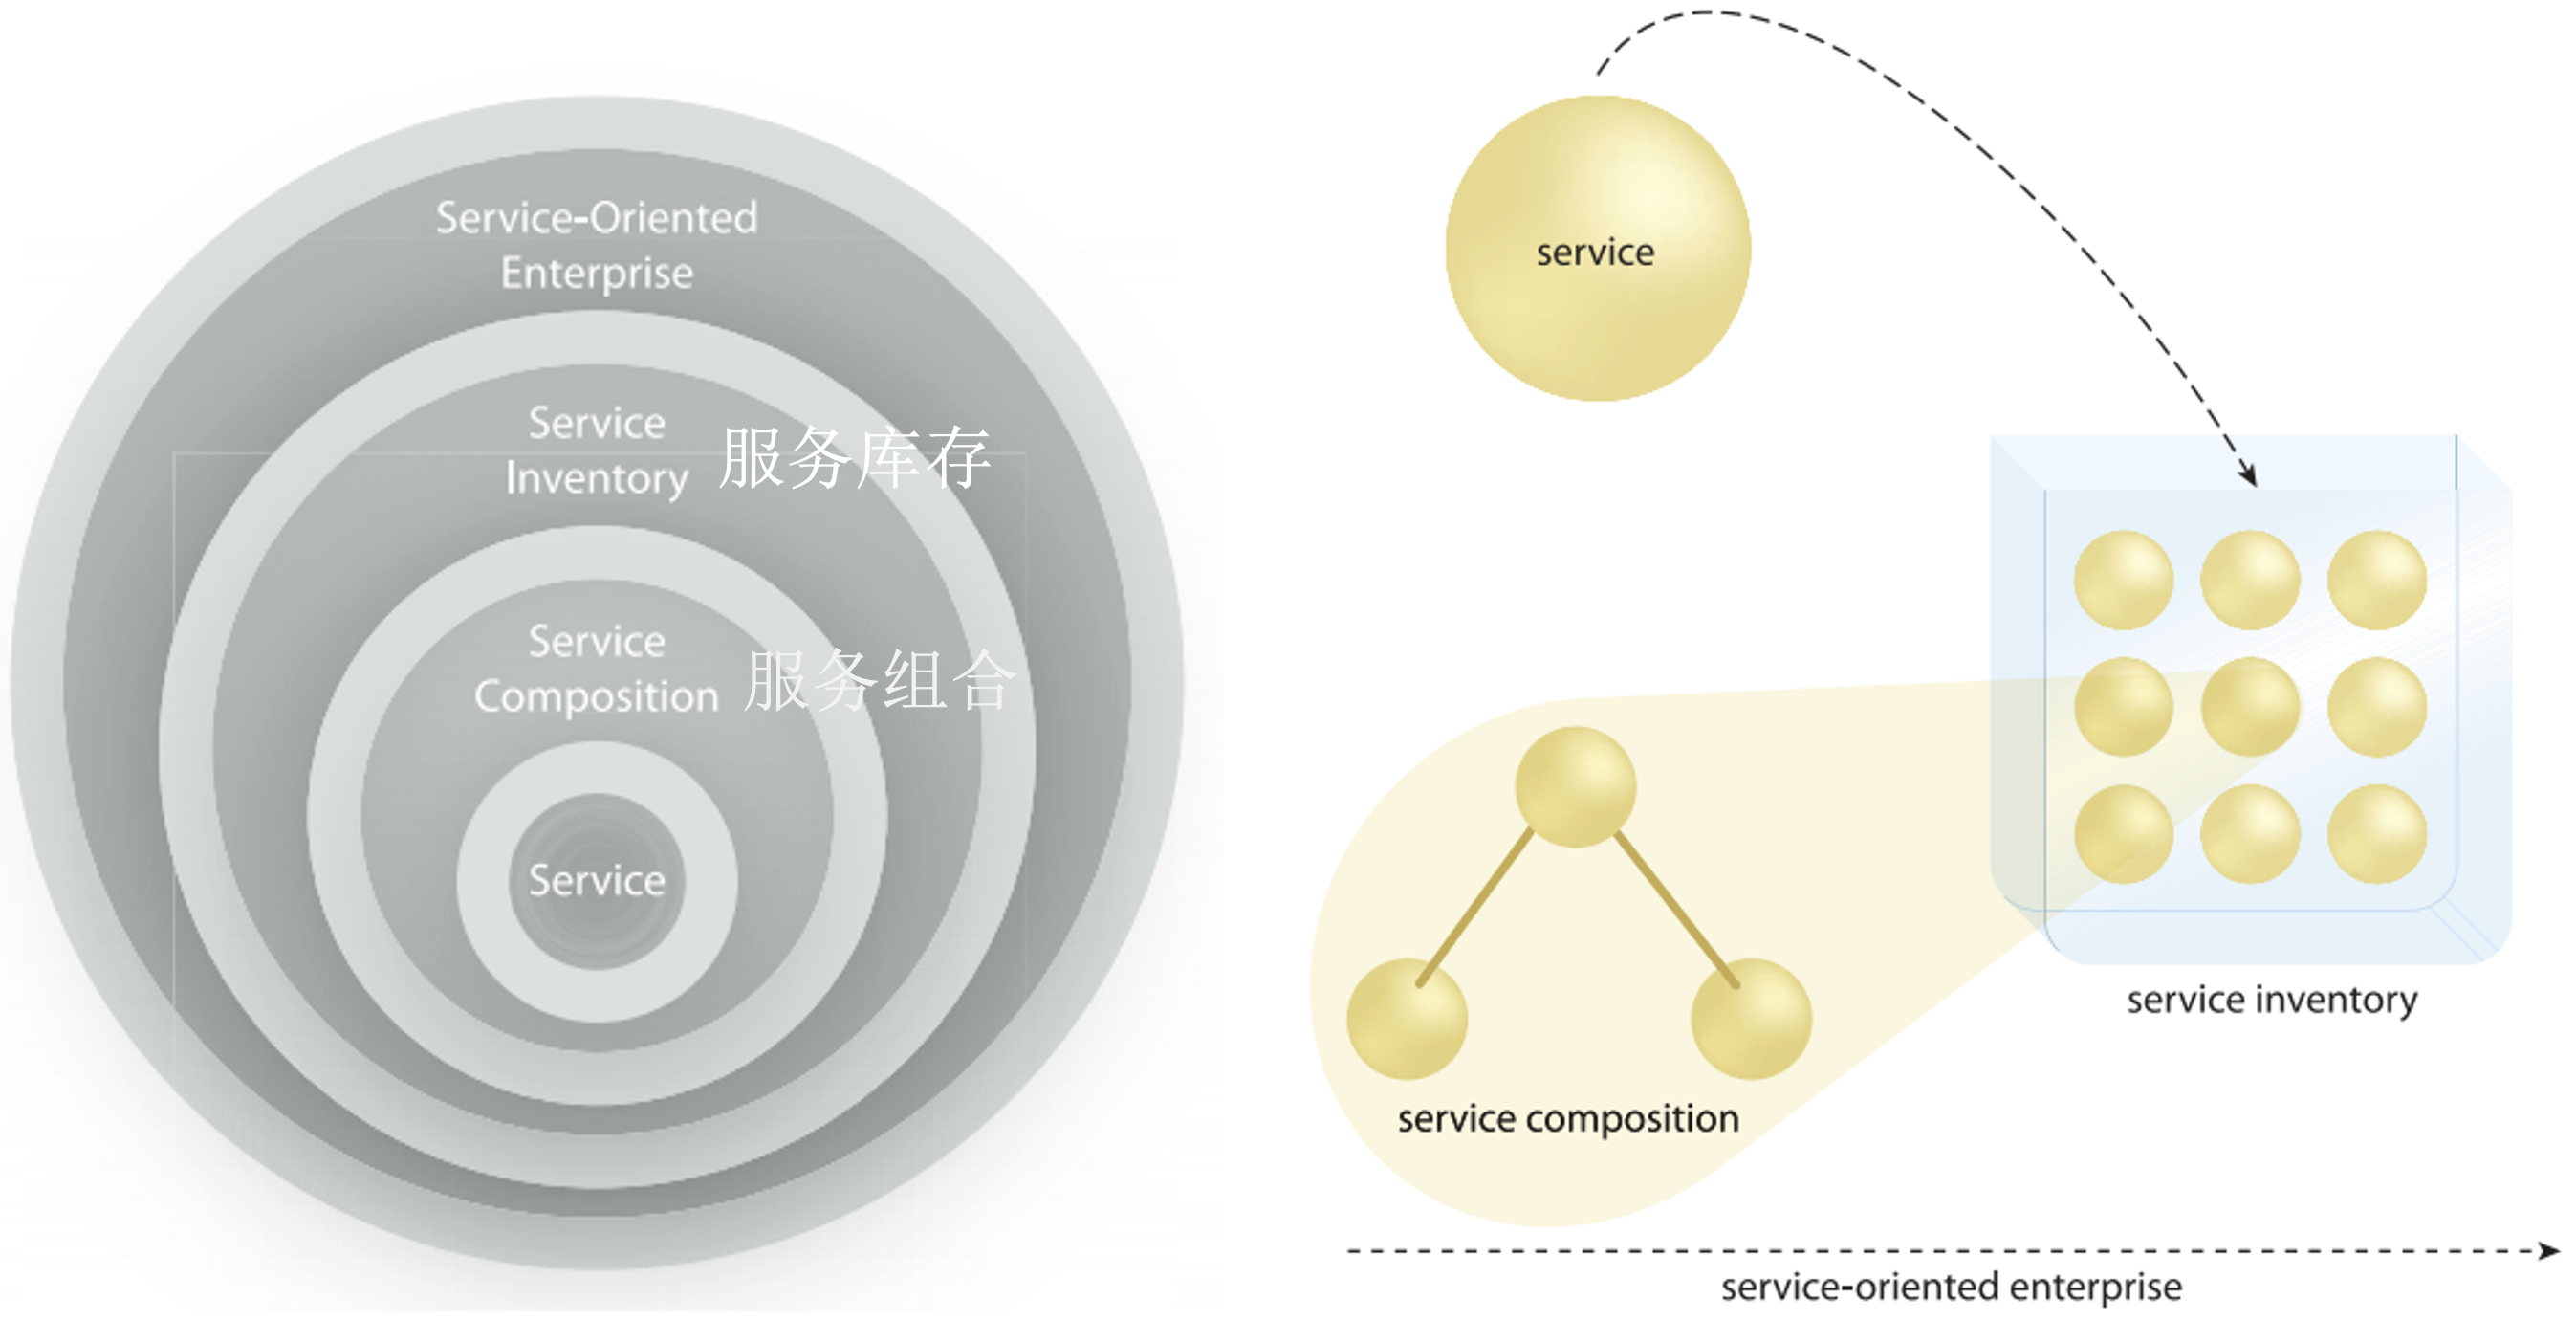
\includegraphics[width=0.8\textwidth]{images/面向服务的应用逻辑.png}
    \vspace{-1em}
\end{figure}

\subsubsection{服务组合}
服务组合由多个装配在一起的服务所构成,用以提供对业务任务或过程进行实现的功能。

由于面向服务倾向于将服务打造为无关的企业资源,一个服务可能被多个消费者程序所调用,它们能在不同的服务组合中组合同一个服务。


\subsubsection{服务库存}
服务库存,是在组织或组织的合理部分边界内一组独立标准化并治理的完备服务。

\begin{figure}[H]
    \vspace{-0.5em}
	\centering
	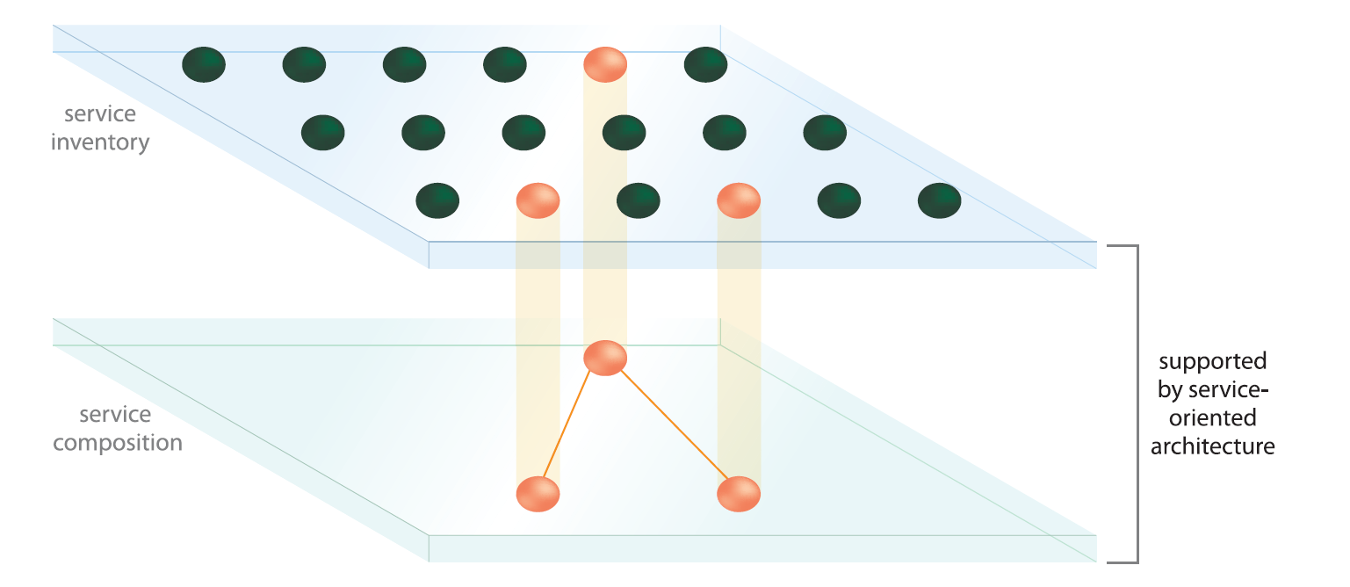
\includegraphics[width=0.8\textwidth]{images/服务库存与服务组合.png}
    \vspace{-1em}
\end{figure}

服务库存可以按照服务模型进行分层:
\begin{itemize}
    \item 应用服务层:紧密和实现相关的较小功能单元抽象出来的服务。
    \item 业务服务层:直接满足调用者、消费者需求的服务
    \vspace{-0.8em}
    \begin{multicols}{2}
        \begin{itemize}
            \item 以任务为中心的业务服务(任务服务)
            \item 以实体为中心的业务服务(实体服务)
        \end{itemize}
    \end{multicols}
    \vspace{-1em}
    \item 编排服务层:(可选的服务层)服务组合的一种实现,一般由领域专家实现,使用平台中立语言(文本化的标记语言,一般为 XML)来描述服务组合的业务逻辑。
\end{itemize}

\begin{figure}[H]
    \vspace{-0.5em}
	\centering
	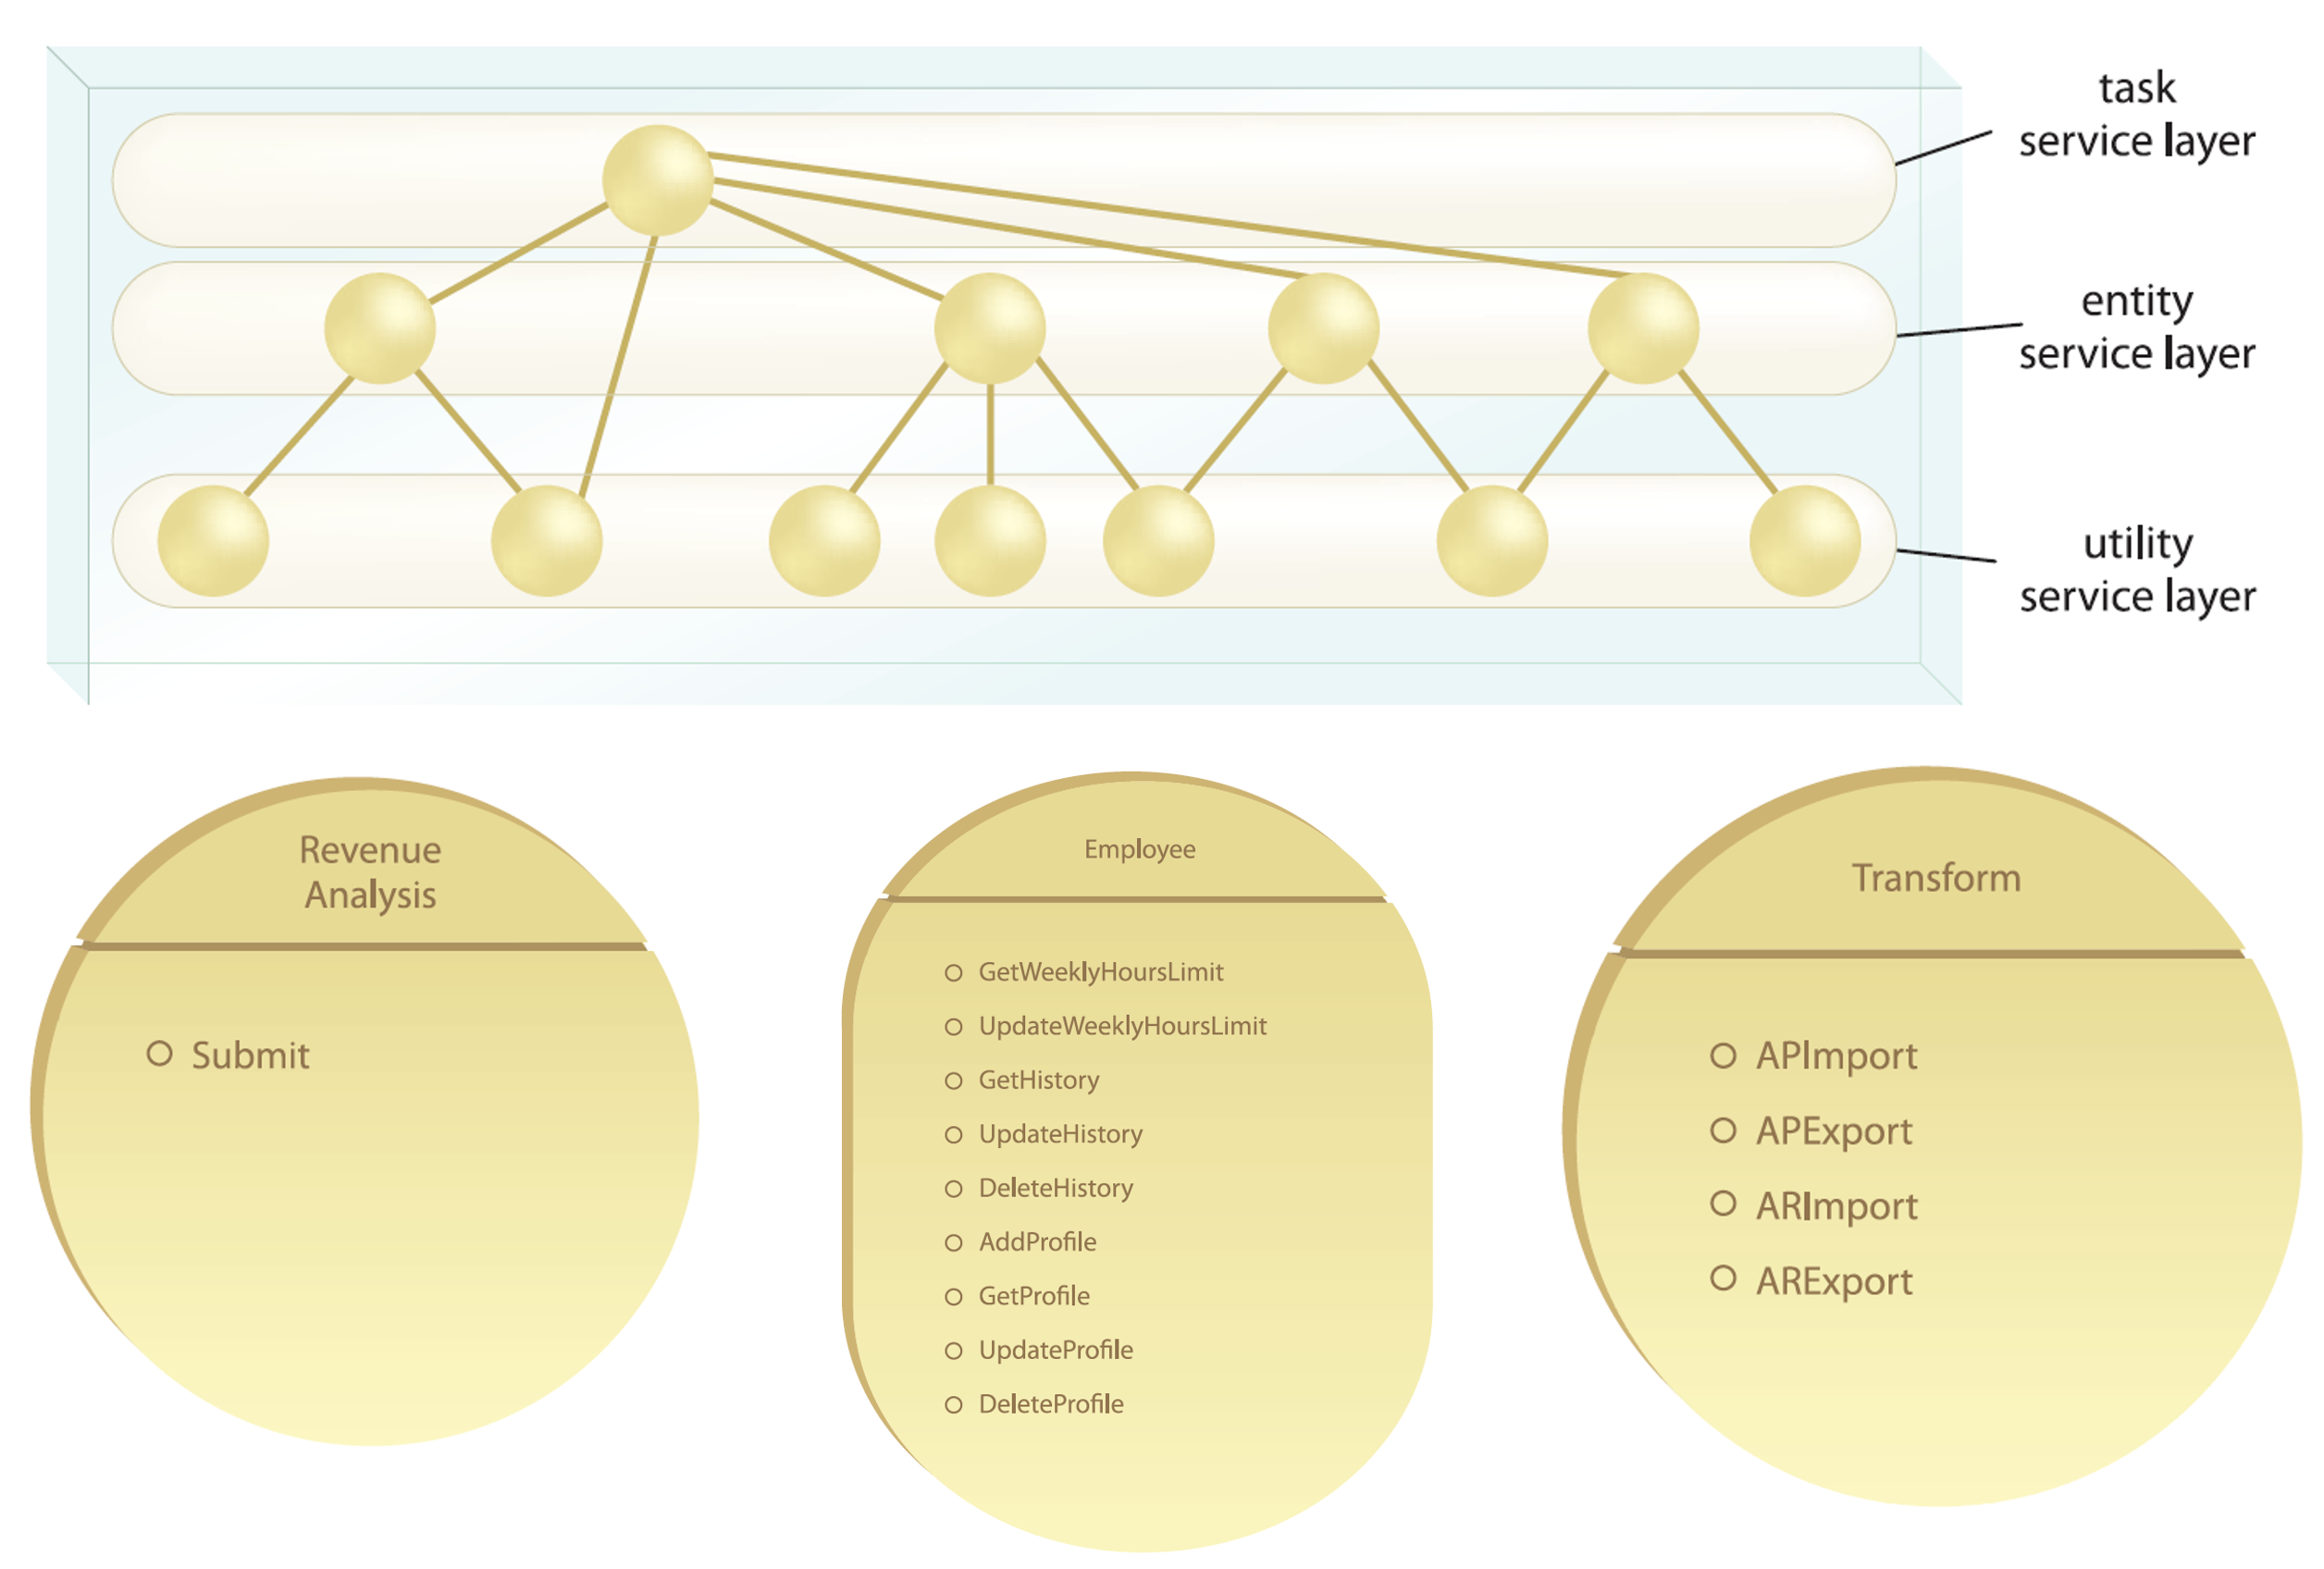
\includegraphics[width=0.7\textwidth]{images/服务模型.png}
    \vspace{-1em}
\end{figure}

在构建前,服务库存的蓝图就已设计完毕了。

服务库存的演化阶段:
\begin{itemize}
    \item 初始服务交付项目(按需开发):服务是中立的,独立于当前软件系统,独立于调用它的服务系统或应用。
    \item 混合应用和成长中的服务库存:服务的数量持续增长,服务组合的可能性也持续增长,但是服务库存仍然尚未完成。
    \item 服务库存基本构建完毕:服务库存的演化基本完成。随着服务库存的增长,潜在的服务组合的复杂度也随之提升。
\end{itemize}


\subsubsection{服务生态系统}
当服务库存按照面向服务的方式进行良好的规划和设计、经过长时间演化、已经基本完备;该组织的服务系统均已合理地转向面向服务的实现,那么该组织内的服务生态系统就被构建起来了。

包含分析、设计、实现、治理、演化等……
\begin{itemize}
    \item 治理:由于共享计算,通过网络以统一的接口调用服务,故需要提供相应的计算资源,来尽量满足所有人的需求。
\end{itemize}
\vspace{-0.8em}
\begin{multicols}{2}
    \begin{itemize}
        \item 兼容性演化:接口不变,后台实现发生变化
        \item 非兼容性演化:接口也需要改变
    \end{itemize}
\end{multicols}
\vspace{-1em}

从消费者角度出发:
\begin{itemize}
    \item 可以被同时、独立调用的,用于满足消费者需求的服务被称为垂直服务(消费者直接调用的服务)。
    \item 垂直服务可以由多个可重用的跨领域的公共服务所构成,这些服务被称为水平服务(不直接被消费者调用的服务)。
    \item 垂直服务和水平服务不是互斥的;二者的区别的唯一标准就在于在某一特定场景下,是否被消费者直接调用。当水平服务被消费者直接调用时,就是也是作为垂直服务。
\end{itemize}


\subsection{服务计算}

\subsubsection{服务计算的定义}
服务计算也叫面向服务的计算(SOC)
\begin{itemize}
    \item 从泛型角度出发:面向服务的计算是一种新型计算泛型。该泛型以服务作为基本概念,以支持快速和低成本开发,和异构环境中分布式应用的灵活组合。
    \item 从软件架构角度出发:面向服务的计算是一组使用面向服务的架构(SOA)来表达计算的概念、原理和方法。在面向服务的架构中,使用带有标准接口的独立构件服务来构造软件应用。
    \item  从服务角度出发:为了在业务服务和IT服务之间建立连接,并进一步改进业务服务,面向服务的计算涵盖了运用计算和信息技术建模、创建、操作和管理业务服务的科学和技术。
    \item 从软件工程的角度出发:面向服务的计算盖了使用服务作为基本抽象元素,采用工程化方法,对服务系统进行分析、设计、开发、测试、部署、管理等活动所涉及的理论、技术和方法。
\end{itemize}

\subsubsection{面向服务与面向服务的目标}
\begin{figure}[H]
    \vspace{-0.5em}
	\centering
	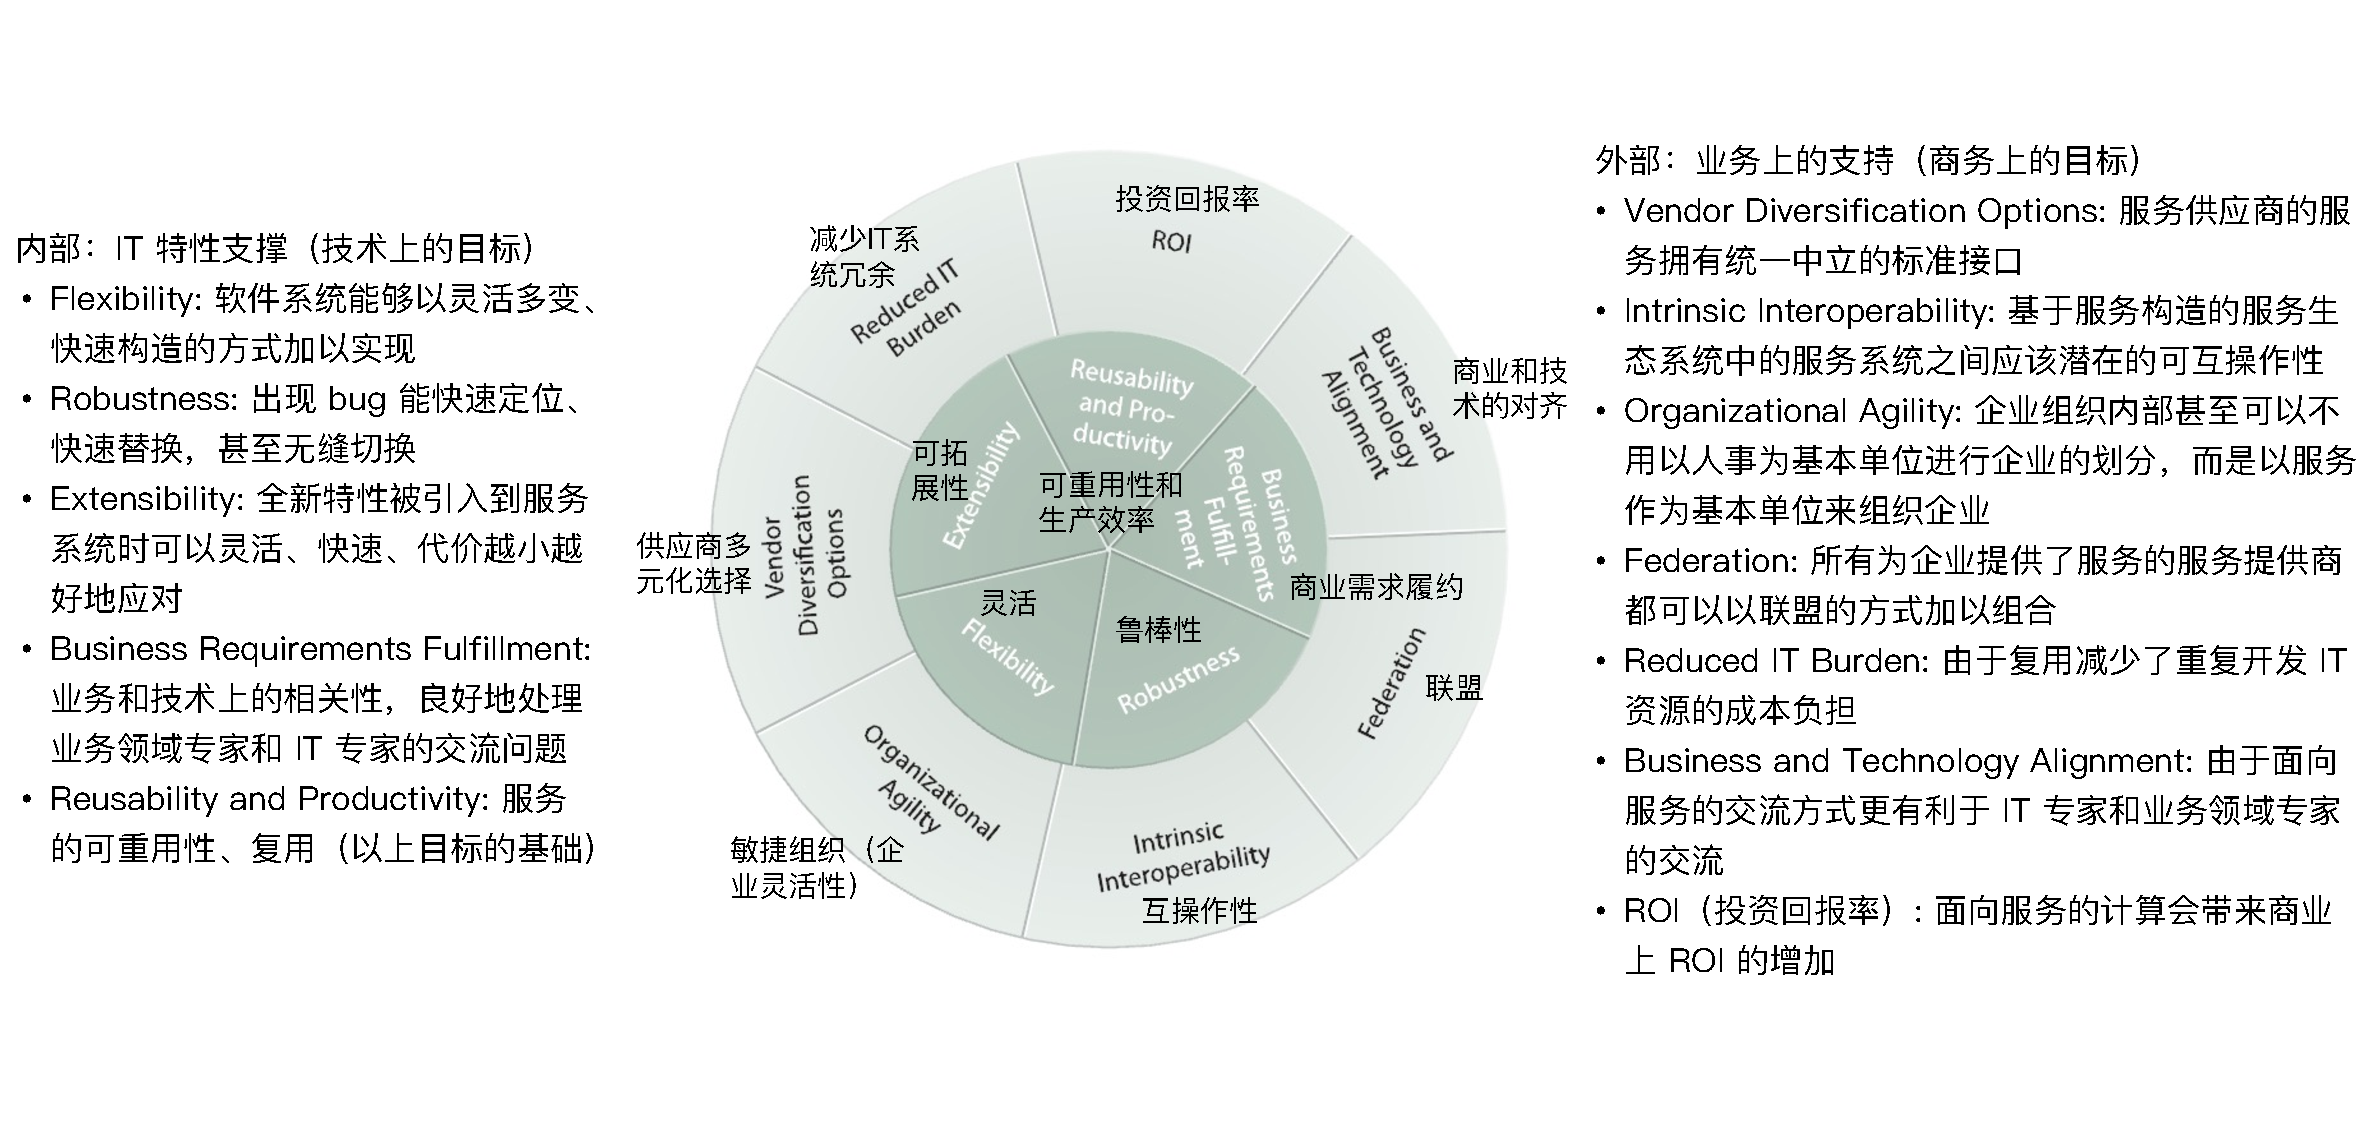
\includegraphics[width=\textwidth]{images/面向服务的目标.pdf}
    \vspace{-2em}
\end{figure}


\subsection{面向服务与面向对象}

\subsubsection{面向服务与面向对象的对比}
\vspace{-0.5em}
\begin{spacing}{1.2}
    \centering
    \begin{longtable}{|m{1.8cm}<{\centering}|m{6.5cm}|m{6.5cm}|}
		\hline
    \textbf{特点} & \multicolumn{1}{c|}{\textbf{面向对象的计算}}                   & \multicolumn{1}{c|}{\textbf{面向服务计算}}                                                          \\ \hline
    方法论         & 通过定义紧耦合的类来进行应用开发;应用架构为基于继承关系的层次式架构;从构造函数——通过类或模型——到系统设计 & 通过定义松耦合的服务来进行应用开发,并将服务组装成可执行的应用;从系统模型到服务模块,从服务抽象定义到服务实现绑定;通过搜索获得可用的服务实现                       \\ \hline
    抽象和协作层次     & 往往由一个团队来负责应用的开发,并负责整个生命周期;开发者必须了解应用领域知识和编程              & 开发任务由三个独立方承担:应用程序开发者,服务提供方和服务代理;其中,应用程序开发者需要了解应用逻辑,但不需要了解具体的服务是如何实现的;服务提供者需要编程能力,但不必了解使用服务的应用 \\ \hline
    代码共享和复用     & 代码复用通过类成员的继承和库函数加以实现。其中库函数在编译时引入,且往往是平台相关的              & 代码在服务层次复用。服务使用标准的结构,并发布在Internet库中。服务是平台无关的,且能够被查找并远程调用。服务代理支持系统的服务共享                         \\ \hline
    动态绑定和重新组合   & 在运行时将名称和方法进行关联。方法必须在应用部署前链接到可执行的代码                      & 在运行时将服务调用和服务进行绑定。可以在应用部署后,再进行服务选定。这一特色使得应用可以在运行时重组                                            \\ \hline
    重组          & 多在设计时决定导入的组件                                            & 可以动态改变应用系统中服务的组合关系,以及服务定义与服务实现之间的绑定关系,即实现动态地添加、修改、删除各个服务节点                                    \\ \hline
    组件通讯和接口     & 与平台和语言有关,例如C++程序难以直接和Java程序通信                           & 与平台和语言无关。组件间通过标准协议通信,如XML,WSDL和SOAP                                                           \\ \hline
    系统维护        & 用户需要时常升级软件,且在执行升级时,应用必须停止                               & 通过互联网升级系统,因为服务多运行在远程服务器上,用户通过互联网进行访问。维护对用户透明                                                  \\ \hline
    可靠性         & 在设计时决定可靠性的方法                                            & 对于服务提供者,每个服务相对简单,更加可靠。对于应用程序存在多个满足同一需求的服务,可用过将故障服务的节点断开并重新绑定到备选服务节点上,获得不间断的应用系统               \\ \hline
    软件拥有        & 软件作为产品销售,为用户所拥有                                         & 软件存在并执行于独立的服务提供商的设备上,用户按照每次对服务使用付费,而不是按照软件产品付费                                                \\ \hline
    \end{longtable}
	\end{spacing}
\vspace{-0.5em}


从设计角度和实现角度来看
\vspace{-0.5em}
\begin{spacing}{1.2}
    \centering
    \begin{longtable}{|m{1.2cm}<{\centering}|m{6.7cm}|m{6.7cm}|}
        \hline
\textbf{特点} & \multicolumn{1}{c|}{\textbf{面向对象的计算}} & \multicolumn{1}{c|}{\textbf{面向服务计算}} \\ \hline
耦合          & 提倡重用和松耦合,但是预先定义的类依赖导致更多的对象紧密绑定        & 服务的松耦合由功能和服务合约给定                     \\ \hline
粒度          & 为支持不同规模的任务,支持细粒度接口(API)               & 鼓励粗粒度的接口(服务描述),通讯消息中包含尽可能多的任务相关信息    \\ \hline
作用域         & 对象作用域更小,更有针对性(往往基于一个软件系统)             & 服务作用域显著不同(往往基于一个服务生态系统)              \\ \hline
前瞻性         & 鼓励处理逻辑与数据的绑定从而产生对象                    & 鼓励创建活动无关的、由消息驱动的服务                  \\ \hline
状态性         & 数据和逻辑的绑定,导致带状态的对象                     & 服务尽可能保持无状态性                          \\ \hline
组合          & 在支持对象组合的同时也支持对象的继承,从而导致紧耦合            & 支持松散耦合服务的组合                          \\ \hline
    \end{longtable}
\end{spacing}
\vspace{-0.5em}

\subsubsection{对象/类/接口与服务合约}
\begin{figure}[H]
    \vspace{-0.5em}
	\centering
	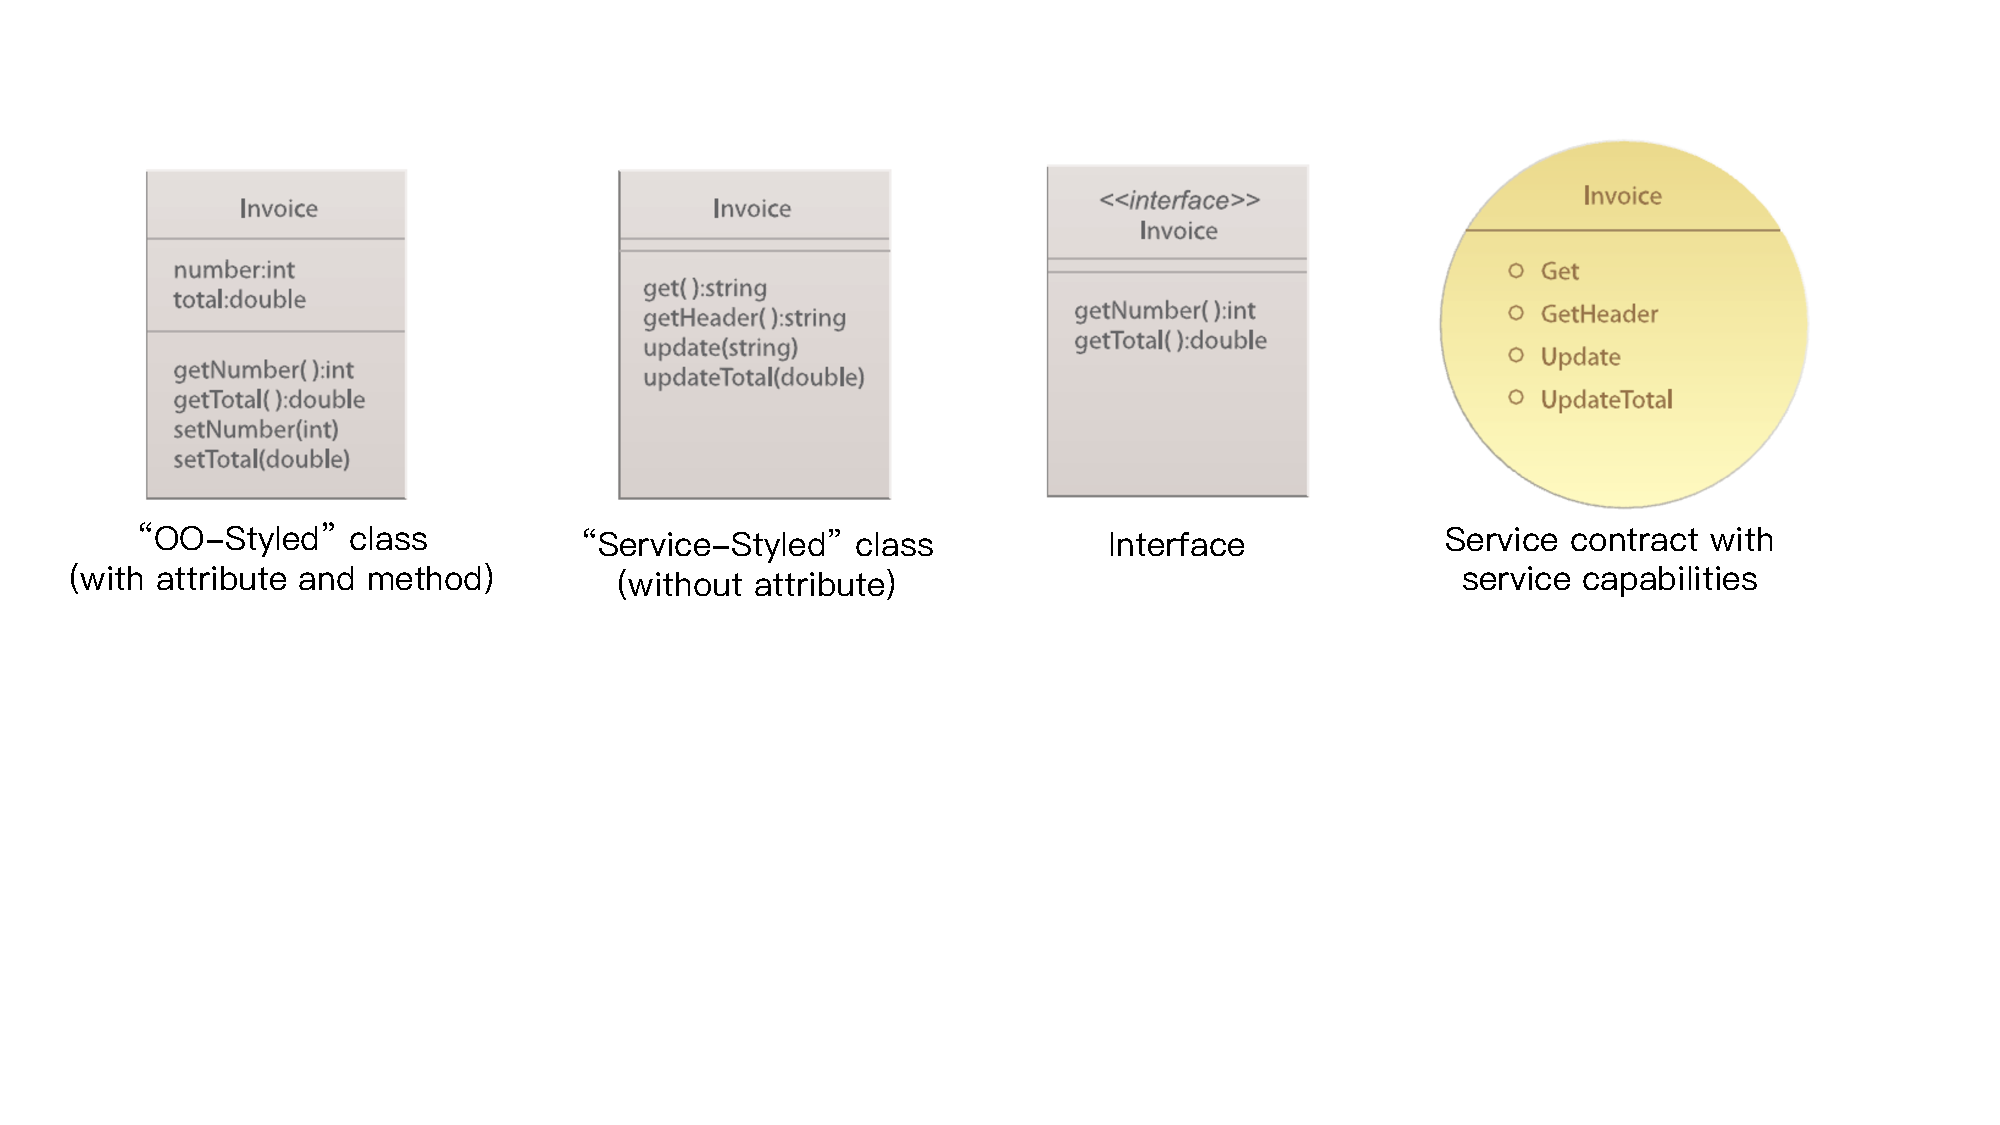
\includegraphics[width=0.8\textwidth]{images/对象、类、接口与服务合约.pdf}
    \vspace{-1em}
\end{figure}

\subsubsection{面向对象设计原则之于面向服务}
面向对象的基本原则
\vspace{-0.8em}
\begin{multicols}{4}
    \begin{spacing}{1.1}
        \begin{itemize}
            \item 封装
            \item 继承
            \item 泛化和特化
            \item 抽象
            \item 多态
            \item 开闭原则
            \item 别重复你自己
            \item 单一职责原则
            \item 委托
            \item 关联
            \item 组合
            \item 聚合
        \end{itemize}
    \end{spacing}
\end{multicols}
\vspace{-1em}

\begin{figure}[H]
	\setcounter{subfigure}{0}
	\centering
	\vspace{-0.5em}	
	\subfloat[封装]{
	\begin{minipage}[t]{0.47\linewidth}
	\centering
	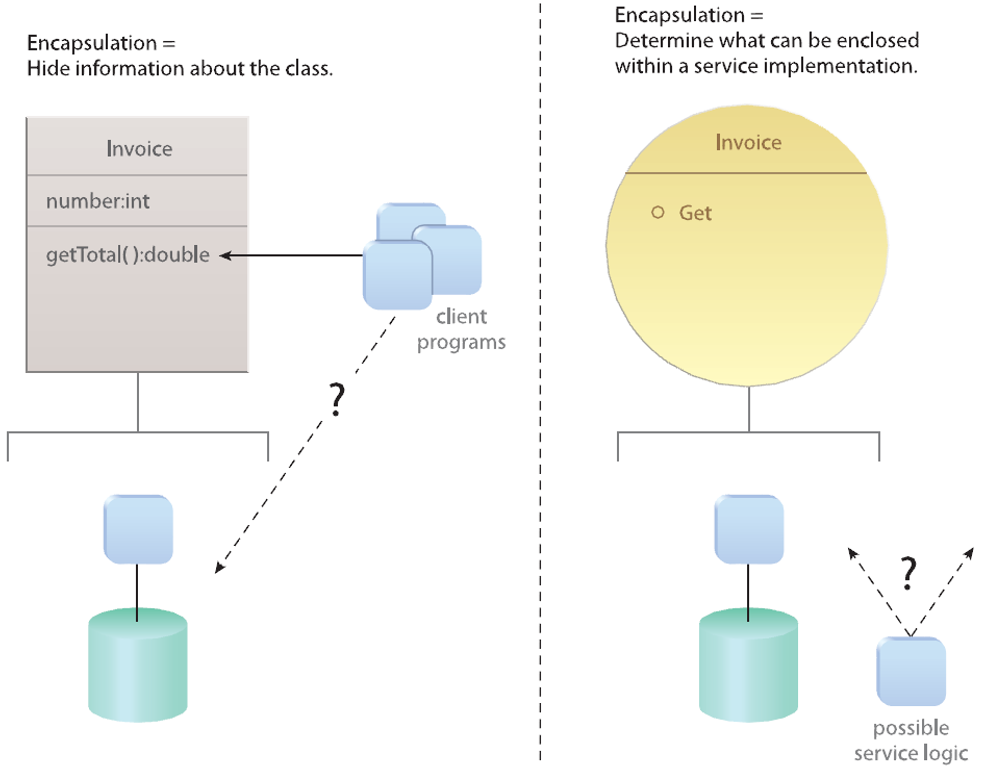
\includegraphics[width=0.97\linewidth]{images/封装.png}
	\end{minipage}
	}
    \hfill
	\subfloat[泛化和特化]{
	\begin{minipage}[t]{0.44\linewidth}
	\centering
	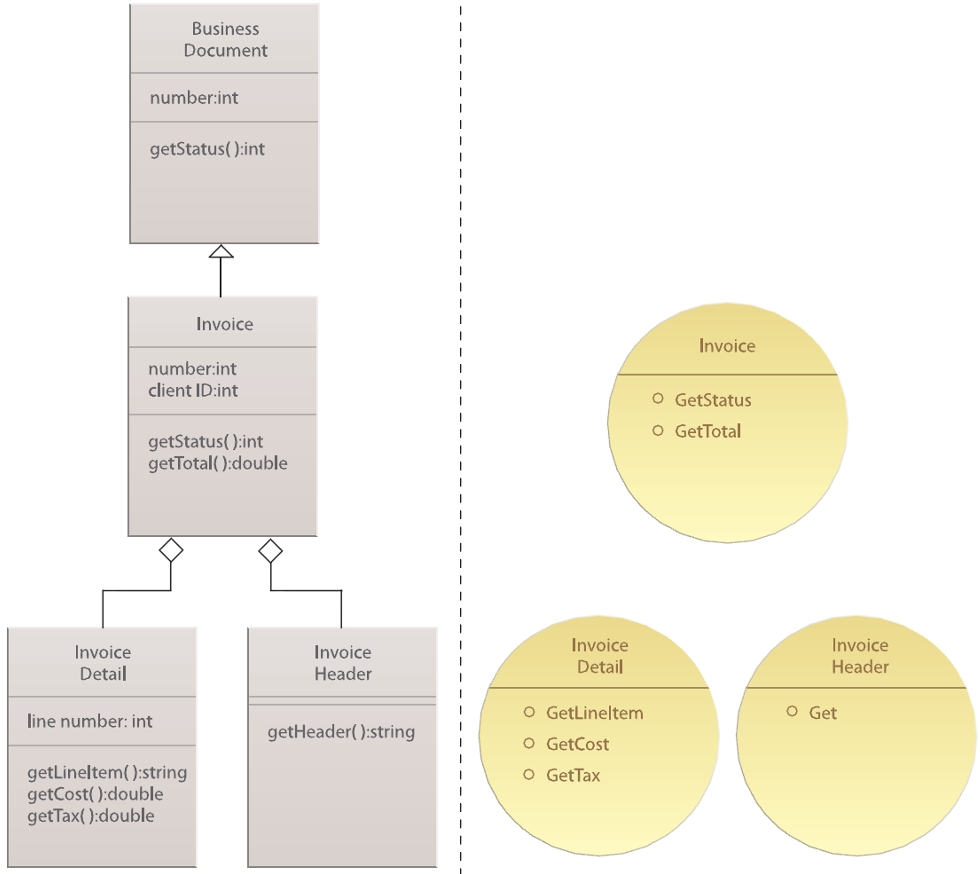
\includegraphics[width=0.97\linewidth]{images/泛化和特化.png}
	\end{minipage}
	}

    \subfloat[抽象]{
	\begin{minipage}[t]{0.31\linewidth}
	\centering
	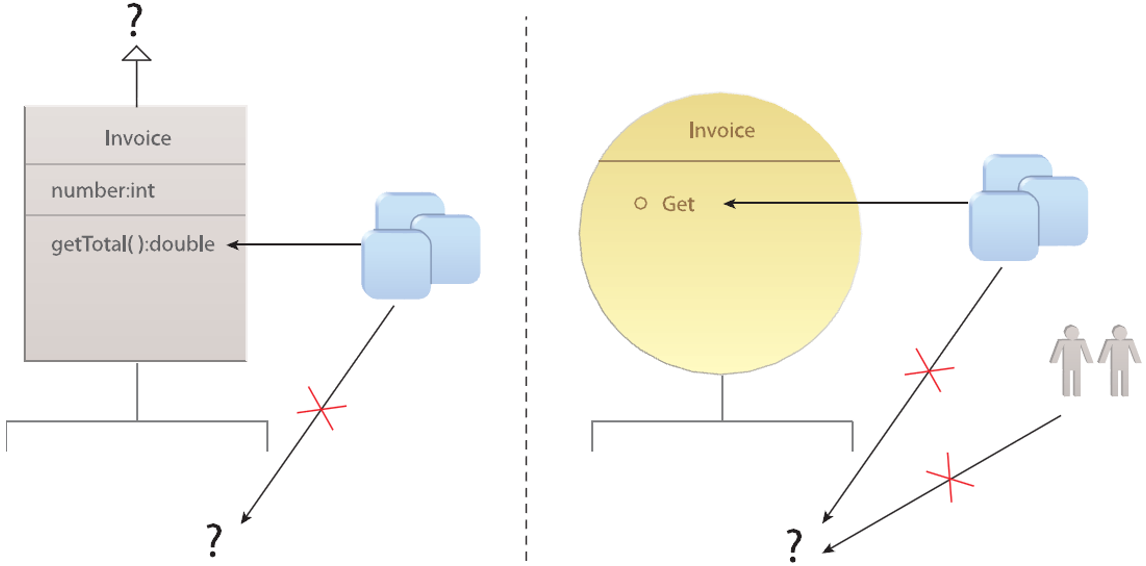
\includegraphics[width=0.97\linewidth]{images/抽象.png}
	\end{minipage}
	}
	\subfloat[继承]{
	\begin{minipage}[t]{0.31\linewidth}
	\centering
	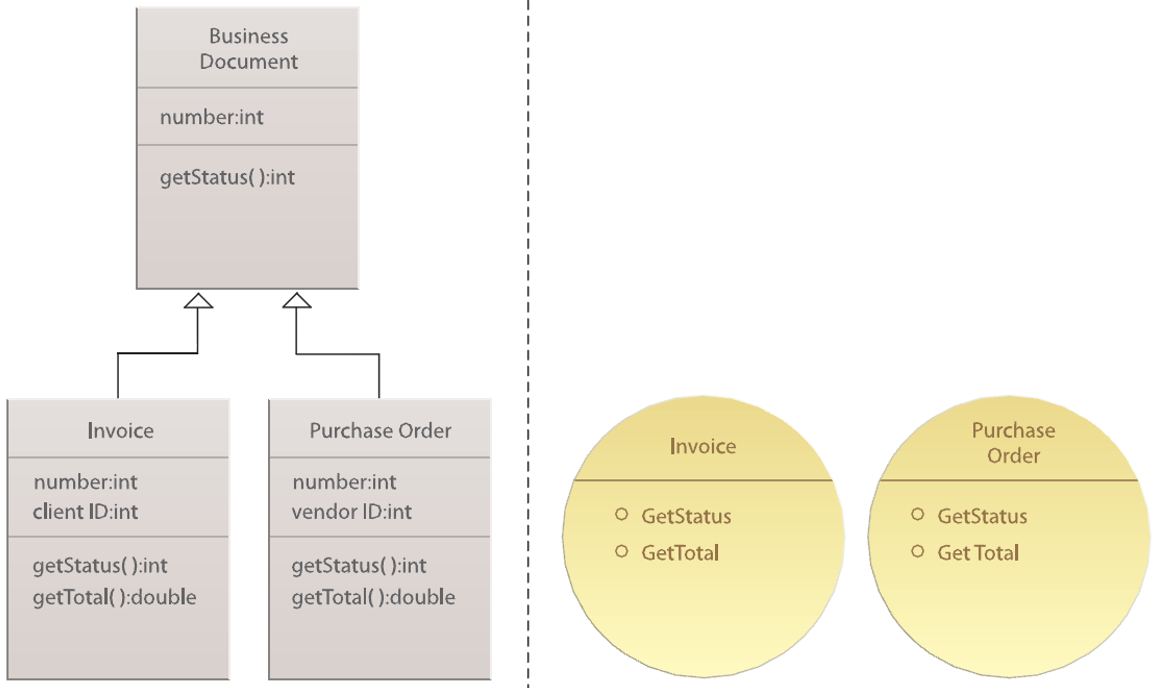
\includegraphics[width=0.97\linewidth]{images/继承.png}
	\end{minipage}
	}
    \subfloat[多态]{
	\begin{minipage}[t]{0.31\linewidth}
	\centering
	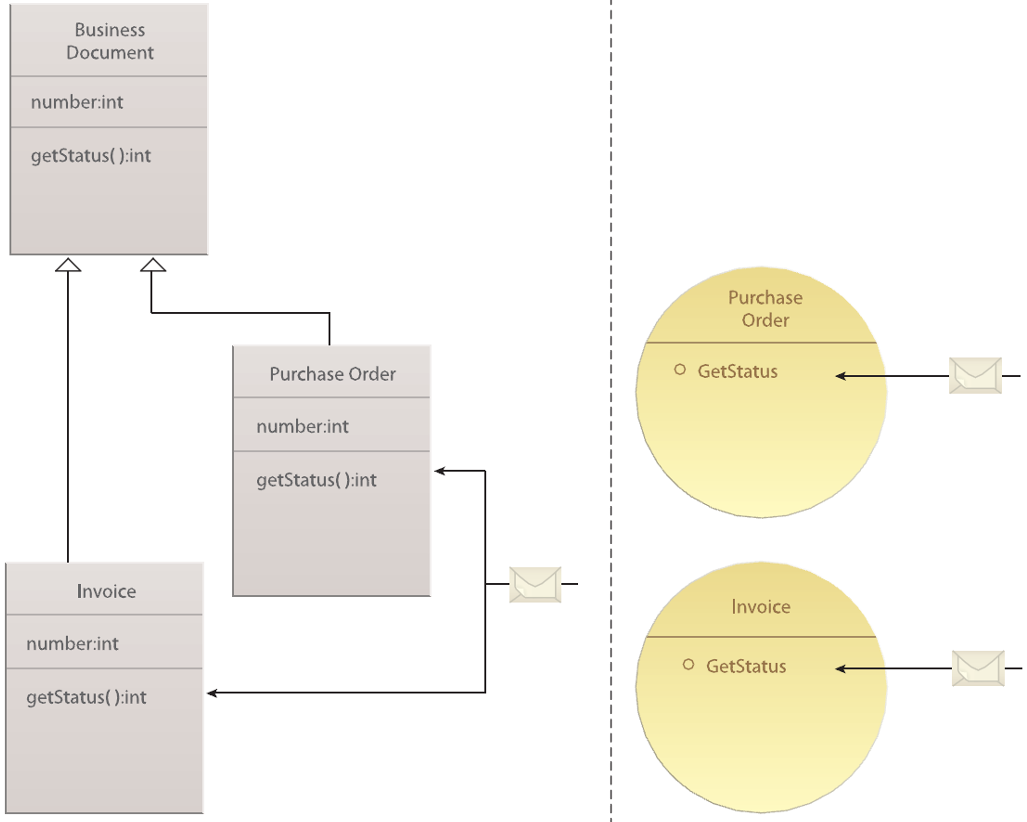
\includegraphics[width=0.97\linewidth]{images/多态.png}
	\end{minipage}
	}
    
	\subfloat[开闭原则]{
	\begin{minipage}[t]{0.53\linewidth}
	\centering
	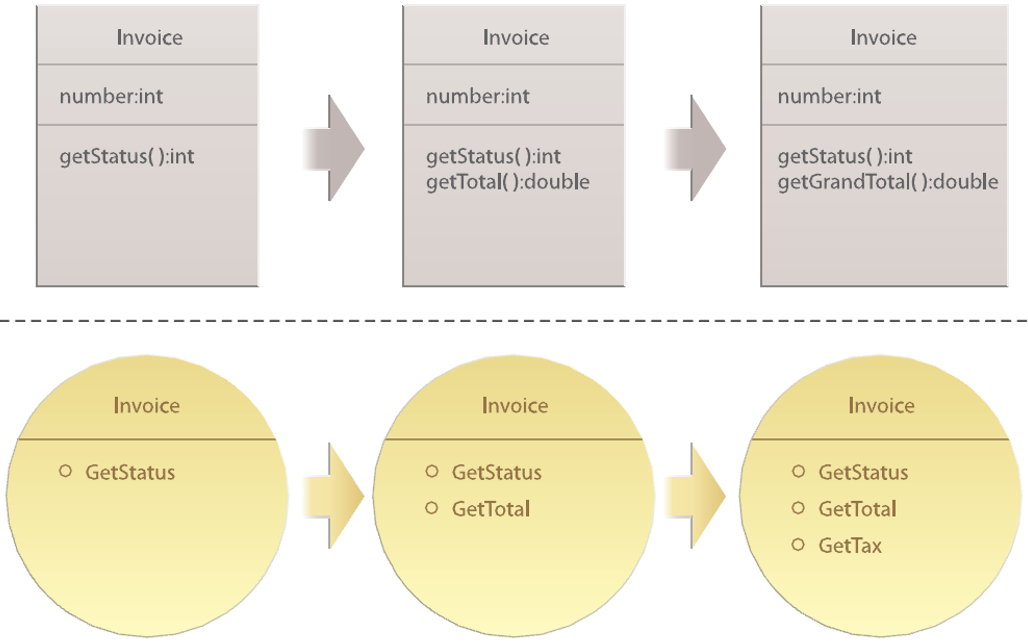
\includegraphics[width=0.97\linewidth]{images/开闭原则.png}
	\end{minipage}
	}
    \hfill
	\subfloat[别重复你自己]{
	\begin{minipage}[t]{0.4\linewidth}
	\centering
	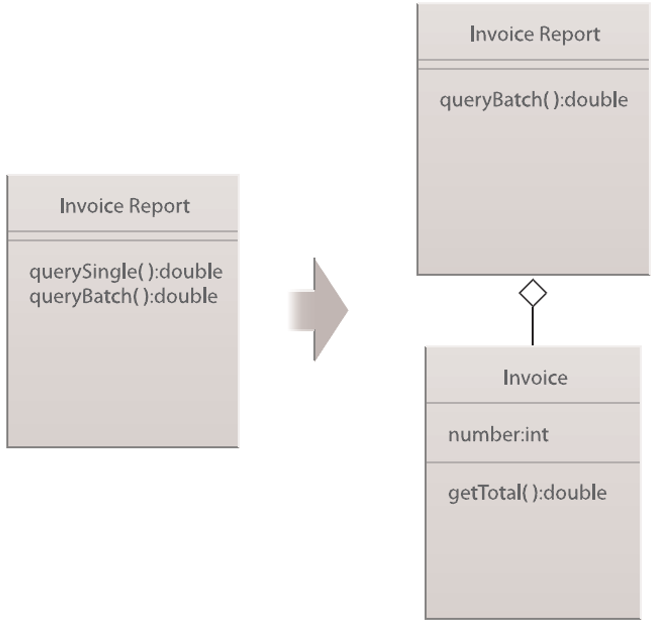
\includegraphics[width=0.97\linewidth]{images/别重复你自己.png}
	\end{minipage}
	}

    \subfloat[委托]{
	\begin{minipage}[t]{0.73\linewidth}
	\centering
	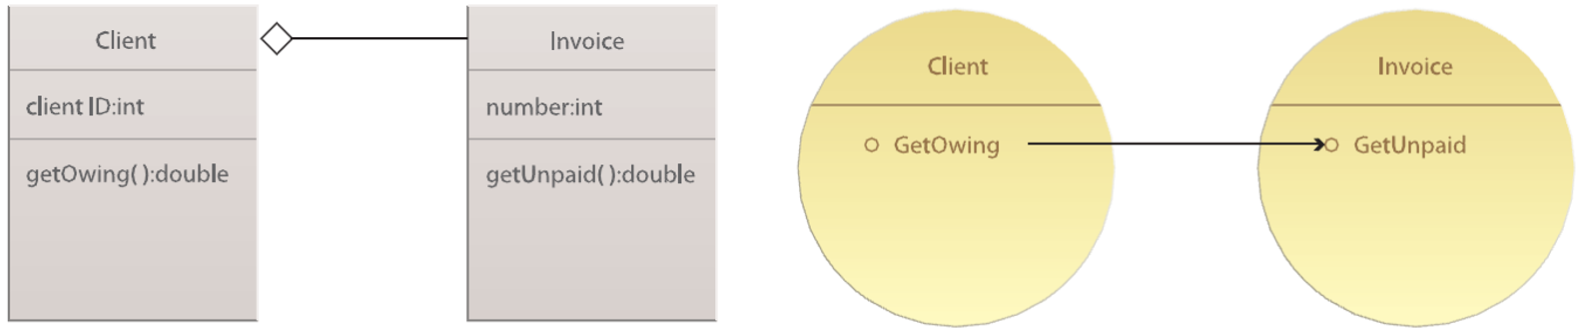
\includegraphics[width=0.97\linewidth]{images/委托.png}
	\end{minipage}
	}
	\centering
	\vspace{-1em}
\end{figure}

\begin{figure}[H]
	\setcounter{subfigure}{8}
	\centering
	\vspace{-0.5em}	
	\subfloat[关联]{
	\begin{minipage}[t]{0.75\linewidth}
	\centering
	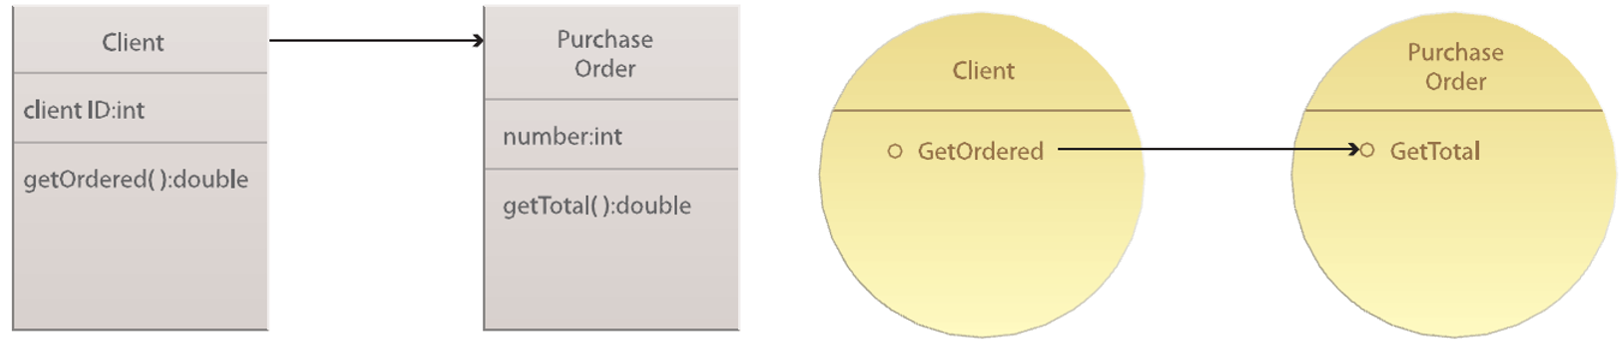
\includegraphics[width=0.97\linewidth]{images/关联.png}
	\end{minipage}
	}

    \subfloat[单一职责原则]{
	\begin{minipage}[t]{0.8\linewidth}
	\centering
	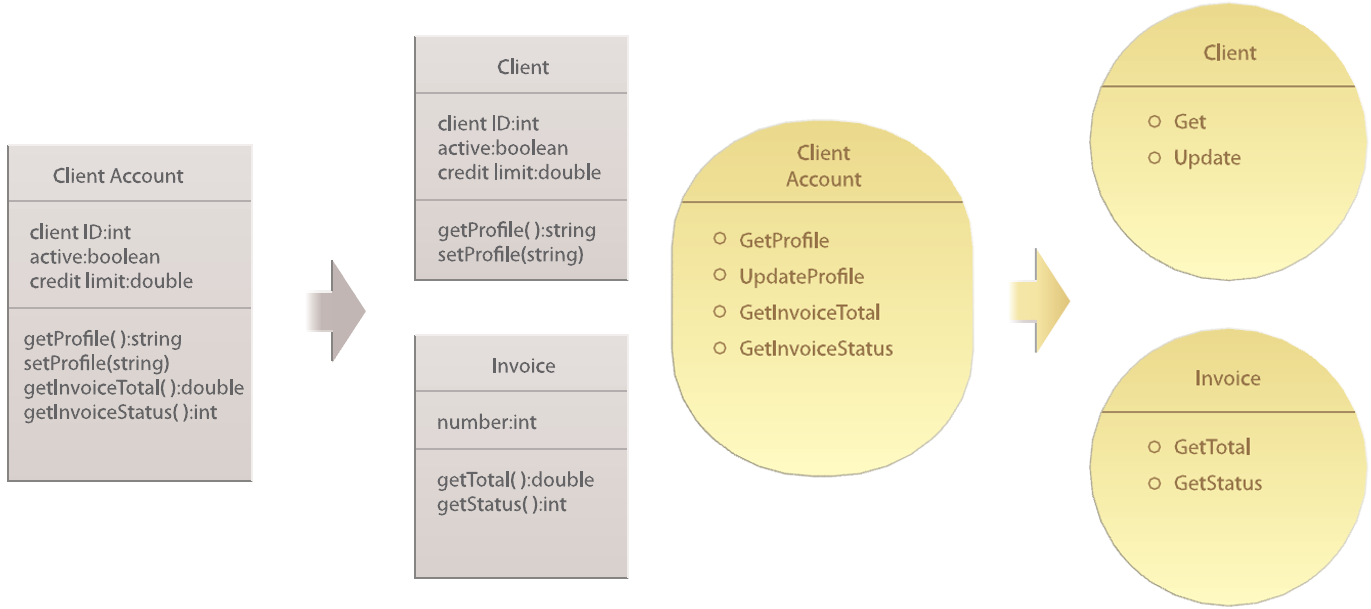
\includegraphics[width=0.97\linewidth]{images/单一职责原则.png}
	\end{minipage}
	}

    \subfloat[聚合]{
	\begin{minipage}[t]{0.47\linewidth}
	\centering
	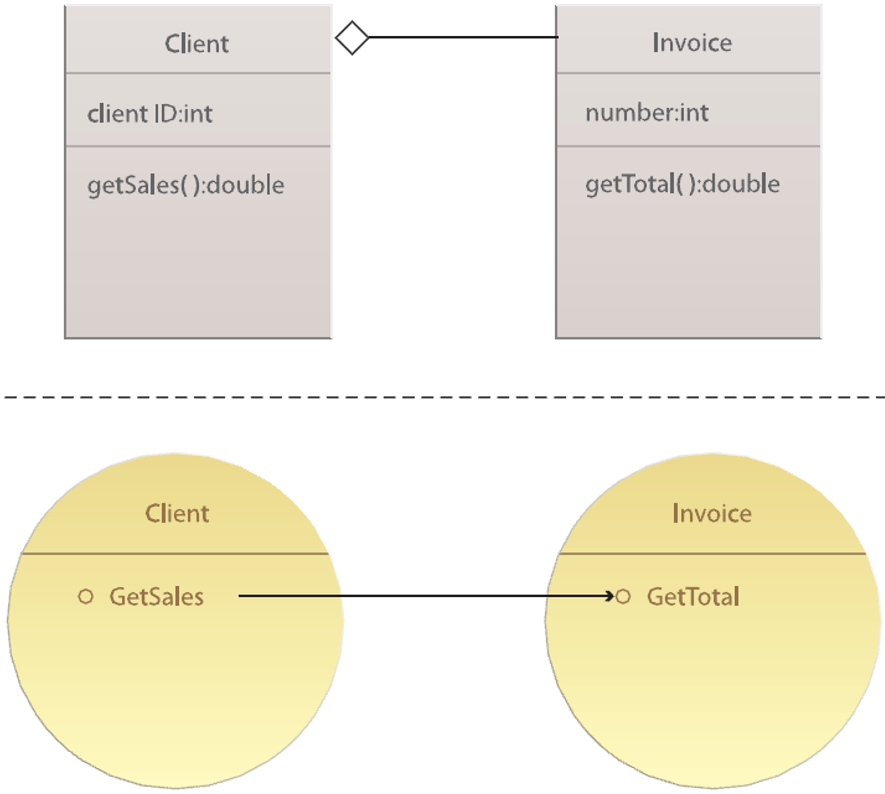
\includegraphics[width=0.97\linewidth]{images/聚合.png}
	\end{minipage}
	}
    \hfill
    \subfloat[组合]{
	\begin{minipage}[t]{0.4\linewidth}
	\centering
	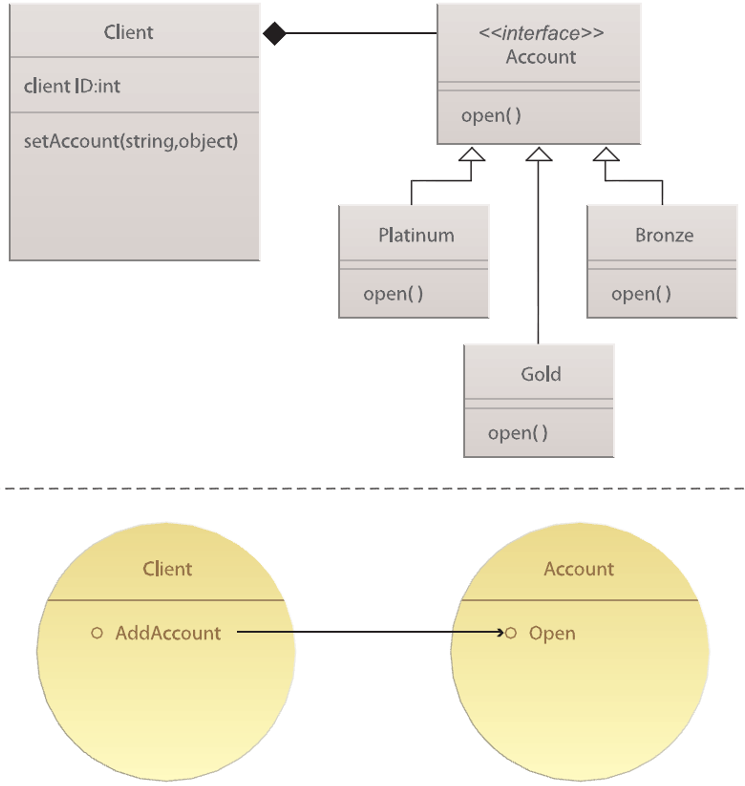
\includegraphics[width=0.97\linewidth]{images/组合.png}
	\end{minipage}
	}
	\centering
	\vspace{-1em}
\end{figure}